\documentclass[a4paper, 11pt]{article}
\usepackage[ngerman]{babel}
\usepackage[utf8]{inputenc}
\usepackage[T1]{fontenc}
\usepackage{amsmath}
\usepackage{amsthm}
\usepackage{amsbsy}

\usepackage{mathrsfs}
\usepackage{amssymb}
\usepackage{amstext}
\usepackage{amsfonts}
\usepackage{float}
\usepackage{graphicx}
\usepackage{esdiff}
\usepackage{hyperref}
\usepackage{geometry}
\geometry{top = 20mm, bottom = 20 mm, left = 25mm, right = 25mm}


\usepackage{setspace}
\onehalfspacing

\usepackage{fancyhdr}
\usepackage{wrapfig}
%\usepackage[hyphens]{url}
%\urlstyle{sf}
%\usepackage[hidelinks]{hyperref}
%\usepackage{breakurl}
%\hypersetup{colorlinks=false}
\usepackage{multirow}
\usepackage[bottom]{footmisc}

%\usepackage{svg}

\title{Mechanik - Erdbeschleunigung mit dem Pendel}
\author{Gruppe 2 \\ \\ Mohammad Bilal Malik \\ Tobias Wild}
\date{\today}

\begin{document}

\begin{titlepage}
	\vspace*{\fill}
	\begin{center}
		\vskip -0.25\textheight
		\vfill
		\newcommand{\Line}{\rule{\linewidth}{0.6mm}}
		\Line 
		{\let\newpage\relax\maketitle}
		\Line 
		\vfill
	\end{center}

	
	\vspace*{\fill}
	\thispagestyle{empty}
\end{titlepage}

\newpage
\thispagestyle{empty}
\tableofcontents
\newpage

%Kopf- und Fußzeile
\pagestyle{fancy}
\fancyhf{}
%Kopfzeile links bzw. innen
\fancyhead[L]{\nouppercase{\leftmark}}
%Kopfzeile rechts bzw. außen
\fancyhead[R]{\thepage}
%Linie oben
\renewcommand{\headrulewidth}{0.5pt}
\fancyfoot[C]{\thepage}


\setcounter{page}{1}

\section{Versuchsbeschreibung}
\subsection{Versuchsziel}
Ziel dieses Versuchs ist die Bestimmung der Erdbeschleunigung mittels des physikalischen Pendels. Dazu wird die Schwingungsdauer des Pendels , die Ausmaße des Pendelkörpers und die Länge der Pendelstange gemessen und daraus die Erdbeschleunigung errechnet.\\

\subsection{Grundlagen}
\subsubsection{Das mathematische Pendel}
Das mathematische Pendel besteht aus einer punktförmigen Masse, die an einem masselosen Faden aufgehängt ist und einer Aufhängung, an der das Pendel reibungsfrei schwingen kann. Luftreibungseffekte werden ebenfalls vernachlässigt. Nach einer Auslenkung um die Ruhelage wird durch die Schwerkraft ein rückstellendes Drehmoment erzeugt, das dazu führt, dass das Pendel eine harmonische Schwingung ausführt. Die Bewegungsgleichung unter der Kleinwinkelnäherung $sin(\phi) \approx \phi$ lautet:


\begin{equation*}
J \cdot \ddot{\phi} = -m_s \cdot g \cdot l \cdot \phi
\end{equation*}

%\begin{figure} [H]
%\centering
%	\includegraphics[scale=0.85]{./Pendel_Bild2.png}
%	\caption[Das mathematische Pendel]{Das mathematische Pendel}
%	\label{pic:Abbildung 1}
%\end{figure}

Durch Einsetzen des Trägheitsmomentes der Masse im Abstand $l$ von der Aufhängung wird die Bewegung unabhängig von der Masse und die Bewegungsgleichung des mathematischen Pendels vereinfacht sich zu: 

\begin{equation*}
\ddot{\phi} = -\frac{g}{l} \cdot \phi = -\omega^2 \cdot \phi
\end{equation*}\

\subsubsection{Das physikalische Pendel}
Möchte man die Erdbeschleunigung empirisch bestimmen, muss das Konzept des mathematischen Pendels jedoch erweitert werden. Dies geschieht vor allem durch die Berücksichtigung der Geometrie und Massenverteilung des Pendelkörpers. Zusätzlich muss gewährleistet sein, dass der schwingende Pendelkörper keinen Einfluss auf die schwingende Stange hat, beide Schwingungen müssen also die gleiche Kreisfrequenz haben.
Sind diese Bedingungen erfüllt, kann man die Vereinfachung auf ein masselos aufgehängten Pendelkörper nutzen. Die Geometrie des Pendelkörpers wird über das Trägheitsmoments des Systems berücksichtigt. Die Erdbeschleunigung $g$ wird dann bestimmt über die Gleichung,

\begin{equation*}
g = \omega^2 \cdot l \cdot (1+\frac{r^2}{2 \cdot l^2})
\end{equation*}\

wobei die $1$ in der Klammer das mathematische Pendel beschreibt und das $\frac{r^2}{2 \cdot l^2}$ der Korrekturterm ist, der die Ausdehnung des Pendelkörpers berücksichtigt. Zur Bestimmung der Erdbeschleunigung werden also 3, von einander unabhängige Messgrößen benötigt.
\newpage

\section{Versuchsaufbau und Durchführung}
\subsection{Aufbau}
Zunächst wird der Versuchsaufbau beschrieben. Auf einem Tisch wird mit Stativmaterial ein Dreifuß mit horizontalen Verbindungsstangen aufgebaut, der möglichst fest steht und selbst nicht mitschwingen kann. Auf einer der horizontal angebrachten Stangen befestigt man einen Winkelaufnehmer, bestehend aus einer Nut, die zusammen mit den Lagerspitzen als Aufhängung des Pendels dient, zwei an der Aufhängung fixierten Permamagneten und einer Hallsonde. Die Hallsonden werden über jeweils 2 Leiterpaare mit dem Cassy-Modul verbunden.\\

%\begin{figure} [H]
%\centering
%	\includegraphics[scale=0.9]{./Versuchsaufbau.png}
%	\caption[Versuchsaufbau]{Versuchsaufbau}
%	\label{pic:Abbildung 2}
%\end{figure}

Wie in 1.2.2 beschrieben, muss darauf geachtet werden, dass die Schwingungsfrequenz der Pendelstange mit Pendelkörper mit der der Pendelstange ohne Körper übereinstimmt. Um das Einstellen der Frequenzen zu vereinfachen, werden 2 Pendel mit zugehöriger Aufhängung und Winkelaufnehmer nebeneinander aufgebaut. An eine der beiden Aufbauten bringt man dann den Pendelkörper an.
\newpage

Die Pendelstangen werden an den Aufhängungen montiert und diese anschließend wie in Abbildung 3 gezeigt über die Lagerspitzen in die Nut des Winkelaufnehmers gesetzt.\\

%\begin{figure} [H]
%\centering
%	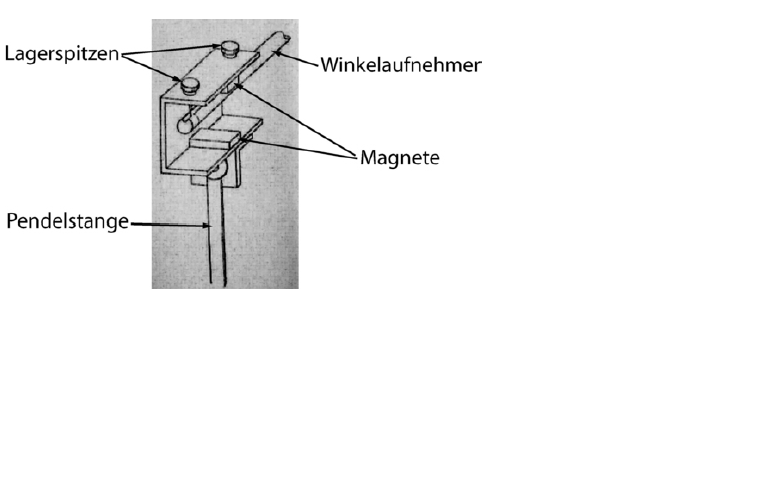
\includegraphics[scale=0.9]{./Winkelaufnehmer.png}
%	\caption[Winkelaufnehmer]{Winkelaufnehmer}
%	\label{pic:Abbildung 3}
%\end{figure}

Die Hallsonden am Winkelaufnehmer messen das Magnetfeld senkrecht zur Nut der Aufhängung. Wird das Pendel ausgelenkt, ändert sich der Winkel zwischen den Permamagneten und der Nut. Die ausgegebene Spannung ist also abhängig vom Auslenkungswinkel des Pendels, bzw. sie ist proportional zum Winkel, wenn darauf geachtet wird, das Pendel nur um kleine Winkel auszulenken. Der Messwert zur Bestimmung der Schwingungsdauer der Pendel ist also die erzeugte Hallspannung.\\


\subsection{Durchführung}
Das erste Ziel besteht darin, die Schwingungsfrequenz des Pendels mit Körper so einzustellen, dass diese mit der Frequenz der Stange allein übereinstimmt. Nur dann darf die oben beschriebene Vereinfachung benutzt werden.
Hierzu werden beide Pendel gleichzeitig ausgelenkt. Die Spannungsverläufe werden über den CASSY-Aufbau parallel aufgenommen und mit der Fast-Fourier-Analyse des CASSY-Labs dargestellt. Die Schwingungsfrequenz des Pendels mit aufgehängtem Körper hängt vom Abstand des Schwerpunkts zum Aufhängepunkt ab. Um also die Frequenz des Pendels einzustellen, wird die Höhe des Pendelkörpers so lange variiert, bis die Frequenz des Pendels ohne Körper getroffen wird. Die Peaks der Fourier-Analyse der beiden Spannungseingänge müssen also aufeinander liegen. 

??

In der Versuchsdurchführung wurde der Angleich der Frequenzen mit der Fast-Fourier-Transformation durchgeführt, das heißt, beide Schwingungsverläufe wurden aufgenommen und die Frequenz des Pendels mit dem Pendelkörper wurde so lange verändert, bis beide Peaks aufeinander liegen. 

??
Ist dies gelungen, darf die Vereinfachung gemacht werden und es folgen die Messungen zu den 3 oben genannten Größen.
\newpage

\subsubsection{Messung der Periodendauer}
Wie oben beschrieben, erfolgt die Messung über die Cassy-Lab-Software. Um die Periodendauer und somit die Schwingungsfrequenz des Pendels zu bestimmen, wird das Pendel um einen kleinen Winkel ausgelenkt und in Schwingung versetzt. Über den Winkelaufnehmer und das CASSY-Modul wird der Spannungsverlauf in der Software dargestellt. Um die Periodendauer genau zu bestimmen, betrachtet man möglichst viele komplette Schwingungen, misst Anfangs- und Endzeitpunkt und teilt anschließend durch die Anzahl der ausgeführten Schwingungen.
\begin{equation*}
T = \frac{t_2-t_1}{n}
\end{equation*}\

Dadurch wird der Fehler der Zeitmessung minimiert (genaueres bei Fehlerrechnung). Um die Anfangs- und Endzeitpunkte so genau wie möglich ablesen zu können, betrachtet man die Maxima/Minima der Schwingung oder die Nulldurchgänge. Bei den Nulldurchgängen ist der Offset zu beachten, der dadurch zustande kommt, dass auch ohne Auslenkung des Pendels eine kleine Hallspannung erzeugt wird. Betrachtet man die Maxima/Minima der Spannungsverläufe, sind die Zeitpunkte dieser unabhängig von der Nulllage des Pendels. \\

\subsubsection{Messung der Pendellänge}
Zusätzlich zur Schwingungsdauert wird zur Berechnung der Erdbeschleunigung die Pendellänge benötigt. Diese wird vom Aufhängepunkt bis zum Schwerpunkt des Pendels gemessen. Dazu wird die Länge der Stange mit dem Maßband und der Abstand der Auflagespitzen zum Ende der Stange mit dem Messschieber bestimmt. Die beiden Werde werden addiert und im Messprotokoll festgehalten. \\

\subsubsection{Messung des Radius des Pendelkörpers}
Ebenfalls benötigt wird der Radius des Pendelkörpers, der im Korrekturterm der Gleichung für $g$ vorkommt und das Trägheitsmoment berücksicht, das durch die Geometrie des Körpers erzeugt wird. Der Durchmesser des Pendelkörpers wird mit dem Messschieber bestimmt und anschließend durch 2 geteilt. \\

\section{Auswertung}
\subsection{Angleich der Frequenzen}
Wie in der Versuchsdurchführung beschrieben wurden die beiden Frequenzen aufeinander angepasst, indem die Peaks mithilfe der FFT aufeinander gelegt wurden. Die Werte der Messreihe wurde aufgenommen und gespeichert. Um eine genauere Aussage darüber zu treffen, ob und vor allem wie genau beide Frequenzen übereinstimmen, werden im ersten Teil der Auswertung beide Periodendauern bzw. Schwingungsfrequenzen mithilfe einer Python-Software bestimmt und miteinander verglichen. Dazu wird jeweils das erste und das letzte Extremum der Messreihen gesucht, die jeweiligen Zeitpunkte abgelesen und mit der oben genannten Formel für $T$ die Periodendauer bestimmt. Aus diesen werden die Frequenzen bestimmt und miteinander verglichen:
\\

%\begin{figure} [H]
%\centering
%	\includegraphics[scale=0.5]{./Frequenzen.eps}
%	\caption[Frequenzverläufe]{Frequenzverläufe}
%	\label{pic:Abbildung 4}
%\end{figure}

\begin{table}[H]
	\large
	\centering
	\begin{tabular}{|c|c|c|}
		\hline 	Nur Stange & Mit Pendelkörper &	Abweichung \\
		\hline	$0,6061$ Hz	&	$0,6587$ Hz		&	$\approx 8\%$ \\
		\hline
	\end{tabular}
	\caption{Anpassung der Frequenzen}
	\label{table:lin_Bereich}
\end{table}
 
Die Abweichung der Frequenzen sollte möglichst gering sein(Größenordnung 0,5\%), da dies sonst bei der Berechnung von $g$ einen Fehler mit sich zieht. Auf unsere Abweichung wird in der Diskussion erneut eingegangen. 

%% HIer noch weiter machen
\subsection{Messreihen}
\subsubsection{Messung der Periodendauer}
Mit der gleichen Methode wie beim Angleich der Frequenzen wird die Periodendauer des Pendels und der jeweilige Fehler bestimmt. Aus der Periodendauer wird die Kreisfrequenz $\omega$ berechnet. Die Ergebnisse mit Fehler lauten:
\\
\begin{equation*}
T = 1,5334s
\end{equation*}\

\begin{equation*}
\omega = 4,0976 \frac{1}{s}
\end{equation*}\


\subsubsection{Messung der Pendellänge}
Das Ergebnis der Messung der Pendellänge setzt sich zusammen aus der mehrfachen Messung der Länge der Pendelstange $l_p$ mit dem Maßband und die Messung des Abstandes Aufhängung-Pendelspitzen $l_a$. Die Werte mit ihren unterschiedlichen Messgenauigkeiten werden addiert. Für die Pendellänge erhält man dann (Mittelwert):
\\
\begin{equation*}
l = l_p + l_a = 0,56926m
\end{equation*}\

\subsubsection{Messung des Radius des Pendelkörpers}
Der Pendelkörper wird mit dem Messschieber bemessen. Wie in der Versuchsdurchführung beschrieben wird der Durchmesser bestimmt und durch 2 geteilt. Das Ergebnis lautet (Mittelwert):
\\
\begin{equation*}
d = 0,07995m
\end{equation*}\
\begin{equation*}
r = 0,039975m
\end{equation*}\

\subsection{Berechnung von g}
Nun wird die gesuchte Erdbeschleunigung $g$ mit den angegebenen Mittelwerten der gemessenen Größen bestimmt, mittels der oben aufgeführten Formel:
\begin{equation*}
g = \omega^2 \cdot l \cdot (1+\frac{r^2}{2 \cdot l^2})   \\  
= (\frac{2\cdot \pi}{T}) ^2 \cdot l \cdot (1+\frac{r^2}{2 \cdot l^2}) = 9,5814 m/s^2
\end{equation*}\

\subsection{Fehlerrechnung}
Die Fehler auf die einzelnen Messgrößen ergeben mit Hilfe des Fehlerfortpflanzungsgesetz zu dem Fehler von $g$.
Zunächst werden die Fehler auf die Längenmessungen betrachtet.
Für die Gesamtlänge $l$ des Pendels ergibt sich aus \begin{equation*}
l = l_a + l_p
\end{equation*}\
folgender Zusammenhang für $\sigma_l $:
\\
\begin{equation*}
\sigma_l = \sigma_{l_a} \oplus \sigma_{l_p}
\end{equation*}\
Mit $\sigma_{l_p}=1mm$ (Messunsicherheit des Maßbandes) und $\sigma_{l_a}=0,05mm$ (Messunsicherheit des Messschiebers) folgt:
\begin{equation*}
\sigma_l = \pm1,00125mm
\end{equation*}
Da mehrere Messungen getätigt wurden, muss der Fehler auf den Mittelwert zur weiteren Berechnung von $\sigma_g$ verwendet werden:
\begin{equation*}
\sigma_{\overline{l}} = \pm0,578mm
\end{equation*}

Der Fehler auf die Bestimmung des Radius ist (unter Verwendung von $\sigma_d=\sigma_{l_a}$, Messunsicherheit des Messschiebers)
\begin{equation*}
\sigma_r = \frac{\sigma_d}{2} = \pm0,025 mm
\end{equation*}
\begin{equation*}
\sigma_{\overline{r}} = \pm0,0144mm
\end{equation*}

Der Fehler auf die Periodendauer ergibt sich aus dem Fehler der Zeitmessung:
\begin{equation*}
\sigma_T = \sqrt{2} \cdot \frac{\sigma_t }{n}
\end{equation*}
wobei es sich bei $n$ ($n=129$) um die Anzahl der Perioden handelt. Mit $\sigma_t = 10 ms $ folgt
\begin{equation*}
\sigma_T = 0,1096ms = 1,096 \cdot 10^{-4} s
\end{equation*}


Für den Fehler auf $g$ lautet das Fehlerfortpflanzungsgesetz:
\begin{equation*}
\sigma_g = \frac{\partial g}{\partial T}\cdot\sigma_T \oplus \frac{\partial g}{\partial l}\cdot\sigma_l \oplus \frac{\partial g}{\partial r}\cdot\sigma_r = \sqrt{(\frac{\partial g}{\partial T}\cdot\sigma_T)^2 + (\frac{\partial g}{\partial l}\cdot\sigma_l)^2+( \frac{\partial g}{\partial r}\cdot\sigma_r)^2} = 
\end{equation*}\
Es werden nun die Summanden seperat betrachtet, gemäß des Praktikumskripts.
\begin{equation*}
(\frac{\partial g}{\partial T}\cdot\sigma_T)^2 = 1,876 \cdot 10^{-6} \frac{m^2}{s^4} 
\end{equation*}
\begin{equation*}
(\frac{\partial g}{\partial r}\cdot\sigma_r)^2 = 2,896 \cdot 10^{-10} \frac{m^2}{s^4} 
\end{equation*}
\begin{equation*}
(\frac{\partial g}{\partial l}\cdot\sigma_l)^2 = 9,373 \cdot 10^{-5} \frac{m^2}{s^4}
\end{equation*}
\begin{equation*}
\sigma_g = \pm9,778\cdot10^{-3} \frac{m}{s^2}
\end{equation*}\



\section{Diskussion der Ergebnisse}
Das Ergebnis für $g$ weicht vom Literaturwert von $g = 9.81 \frac{m}{s^2}$ ab. Der am schwersten gewichtete Fehler kommt durch die relativ ungenaue Messung der Länge des Pendels, da diese unter anderem mit dem Maßband und einer Genauigkeit von $1mm$ bestimmt wird. Die Zeitmessung für die Periodendauer bringt ebenfalls einen Fehler mit sich, der aber im Vergleich relativ klein ist, da man mehrere Perioden vermisst und den Fehler dadurch minimieren kann. Der dritte Fehler der Messung ist zu vernachlässigen, da der Radius des Pendelkörpers nur mit dem Messschieber und somit einer viel höheren Genauigkeit bestimmt wird. Außerdem ist das Verhältnis von Pendellänge zu Radius des Pendelkörpers im Quadrat so klein, dass der Fehler auch ohne das genaue Messen deutlich weniger Einfluss auf das Ergebnis für g hat als die anderen beiden Fehler. 
Ein zusätzlicher Fehler kommt dadurch zustande, dass man vor Beginn der Messung die beiden Frequenzen aneinander anpassen muss, und das über die Fourier-Analyse nur bis zu einer bestimmten Genauigkeit funktioniert. Die beiden Frequenzen liegen also nicht exakt aufeinander sondern weichen minimal voneinander ab.
\end{document}